\documentclass[11pt,a4paper]{article}
\usepackage[utf8]{inputenc}
\usepackage[english]{babel}
\usepackage{amsmath}
\usepackage{amsfonts}
\usepackage{amssymb}
\usepackage{graphicx}
\graphicspath{{../figures/}}
\author{Jacob Heden Malm}
\title{DD2424 Assignment 2}
\begin{document}
\maketitle

\section{Analytic gradient computations}
Since I wrote my code in python I could not use the provided ComputeGradsNum() method. Instead I performed the sanity check as specified in the lab instructions to check that my gradient computations were correct. I wrote a method called sanity\_check() where I passed in 100 data points and attempted to get my loss values as low as possible. I did this by training on the entire batch of data passed in for 1000 epochs and monitoring the development of the loss values.\\

Here is an example of the development of the loss values through training on this very limited data set.

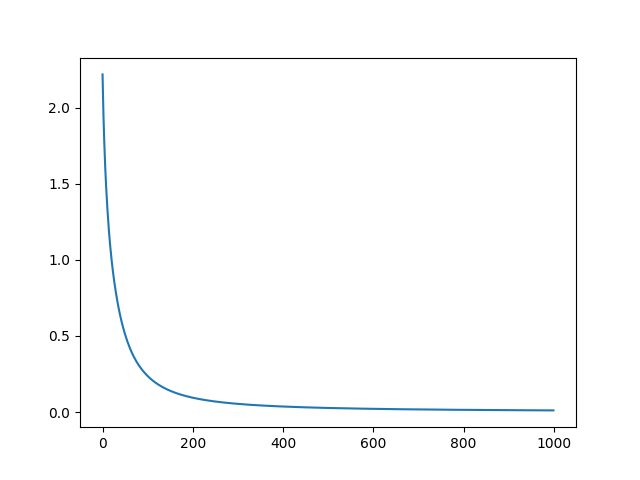
\includegraphics[width=\textwidth]{sanity_check.png}

The shape of the development of the loss function is almost exactly what we'd expect a nice satisfying 1/x curve. This suggests, since the derivative of this curve is logarithmic, that the rate of improvement decreases the more we have already learned, which makes sense. We also manage to get almost arbitrarily close to 0, suggesting that the network learns to recognize the training set perfectly, which allows us to conclude that the gradient computations are in fact working.


\section{Cyclical learning rate on a single batch of data}
The cost and accuracy of our network trained with step size = 500, trained for one cycle look as follows:

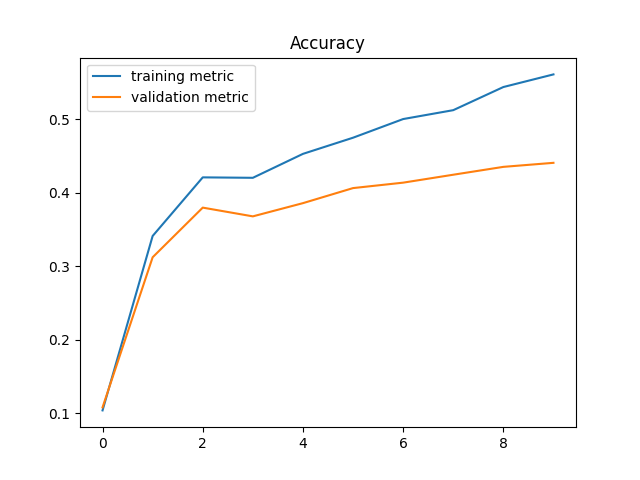
\includegraphics[width=\textwidth]{ns=500_accuracy.png}
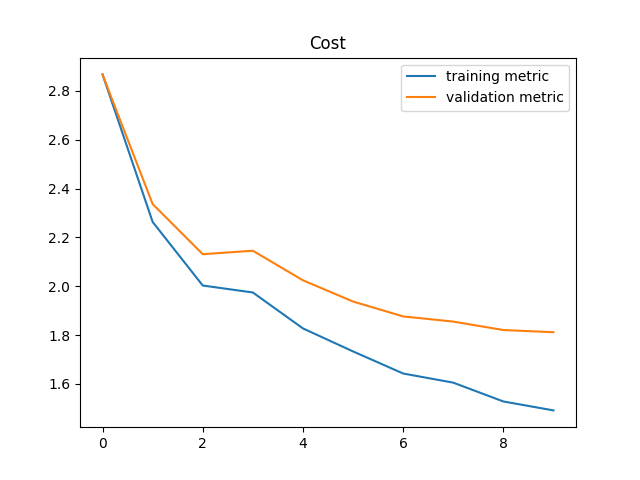
\includegraphics[width=\textwidth]{ns=500_cost.png}

Here we can see that the loss and accuracy are almost monotonically decreasing/decreasing throughout a cycle. We also see that for this data/regularization parameter setting there is a moderate degree of overfitting. Here, lambda is as specified 0.01.\\

This is how the graphs look when we increase the stepsize to 800, and also train for 3 complete cycles.

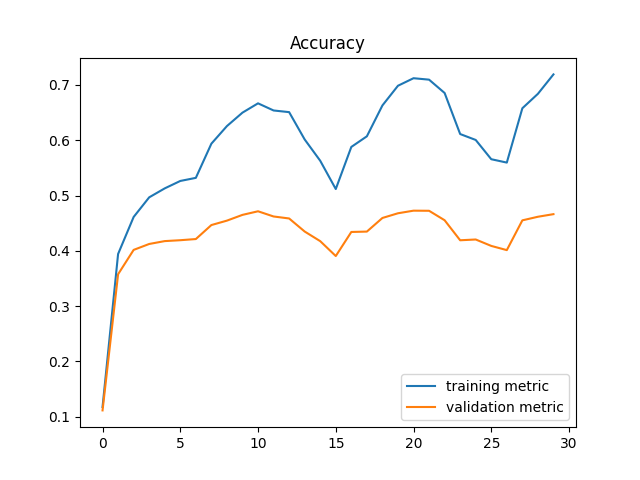
\includegraphics[width=\textwidth]{ns=800_accuracy.png}
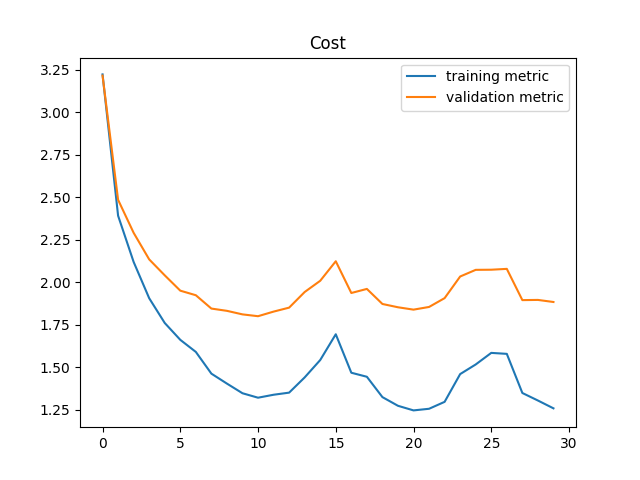
\includegraphics[width=\textwidth]{ns=800_cost.png}

Here we can clearly see the cycle of learning rate reflected in the graphs. One cycle of learning rate carries with it both an increase and decrease in cost and accuracy, however as specified in the instructions, if we cut off the training at the end of one of these cycles we are able to "time" the conclusion of training at a point where our learned weights are optimal.

\section{Coarse search}

I first performed a coarse random search for the optimal $\lambda$ settings. I tried 10 different lambda samples uniformly sampled from the range 1e-5 and 1e-1, trained for 2 cycles each. The accuracy of these settings on the validation set are shown here:

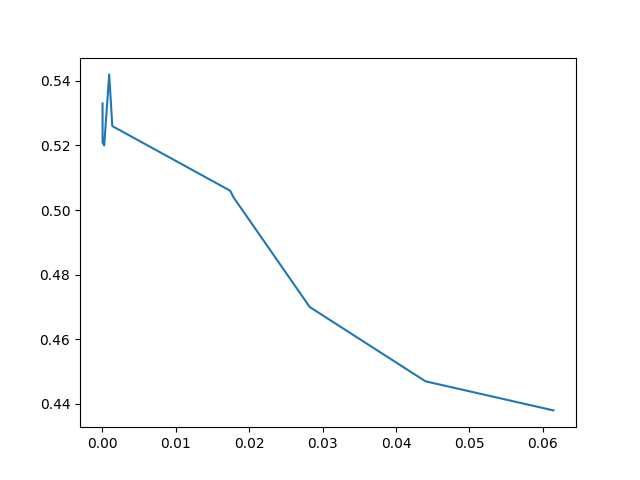
\includegraphics[width=\textwidth]{coarse_search.png}

The 3 best performing $lambda$ values were 1.09e-05,0.00091, and 0.0013. In general, outside of this neighbourhood the performance decreased monotonically. This suggests that we should concentrate our fine search in the vicinity of these points.


\section{Fine search}

I performed the fine search by assessing accuracy on 30 samples for the $\lambda$ parameter sampled uniformly between 1e-5 and 1e-3. The accuracy on the validation set is shown here:


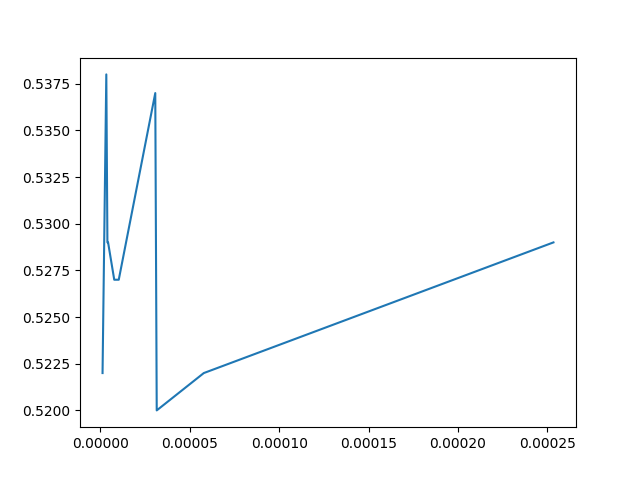
\includegraphics[width=\textwidth]{fine_search.png}

We can see that the relationship between lambda and performance is not as easy to assess here. In general, we reach high values when lambda is very small, but there is a large degree of variance here, and then as lambda increases at first performance decreases, until we reach roughly 0.0007, where it peaks again. The 3 highest values for lambda found were 0.0009, 3.3e-5, and 0.00072. 


\section{Highest performing network}
I chose $\lambda$ to be 0.0009 based on my random searches for hyperparameter settings. I used a hidden layer of 60 nodes, and 5 cycles of training to train my highest performing network. The graphs can be seen here

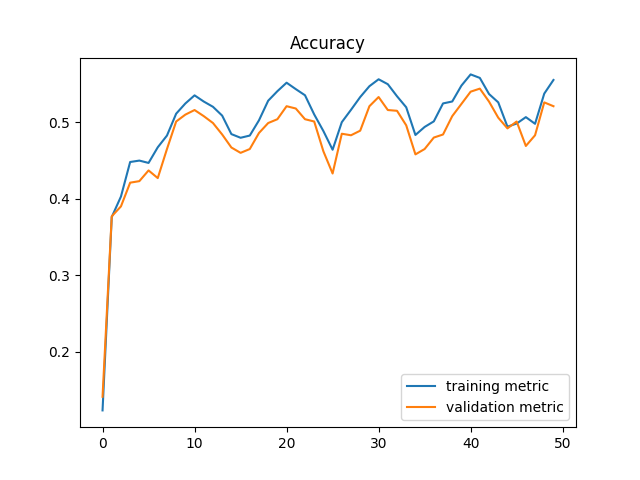
\includegraphics[width=\textwidth]{best_network_accuracy.png}
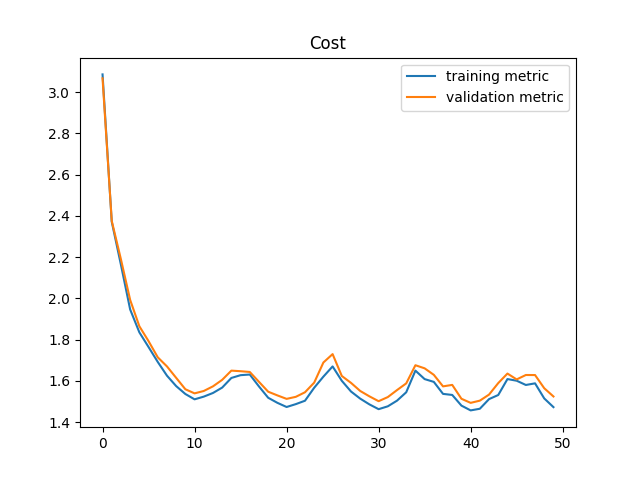
\includegraphics[width=\textwidth]{best_network_loss.png}

The best networks final accuracy on the test set was: 0.5263333333333333.


\end{document}
